\documentclass[8pt]{beamer}
\mode<presentation>
{
  \usetheme{Madrid}
  \usefonttheme{default}
}
\renewcommand{\baselinestretch}{1.5}
%\usepackage[legalpaper, landscape, margin=2in]{geometry}
\usepackage[utf8]{inputenc}
\usepackage[T1]{fontenc}
\usepackage{graphicx}
\usepackage{tikz}
\usepackage{circuitikz}
\usepackage{hyperref}
\usepackage{listings}
\usepackage{multicol}
\setlength{\columnsep}{4.5cm}

\title[Report]{A Fourier Perspective on Model Robustness in Computer Vision}
\author{Krishna Srikar Durbha}
\date{21st October 2020}

\begin{document}

\begin{frame}
  \titlepage
\end{frame}

\begin{frame}
\frametitle{Table of Contents}
\tableofcontents
\end{frame}

\section{Introduction}
\begin{frame}[allowframebreaks]{Problem with Distributional Shift}
\textbf{Distributional Shift:}\\
\qquad If Train and Test sets are not from the same Distribution such a shift is called Distributional Shift. Covariate Shift may be the most widely studied. We assume that while the distribution of inputs may change over time, the labeling function, i.e., the conditional distribution $P(y|\textbf{x})$  does not change. Statisticians call this Covariate shift because the problem arises due to a shift in the distribution of the Covariates (features).

\vspace{0.25in}

\textbf{Example:}\\
\qquad If Model is trained on Images from Fig.\ref{fig:Train Images} and when test on Images from Fig.\ref{fig:Test Images}. There is a substantially difference in characteristics between the Train and Test Set as Training Set contains Real-World Images while Test set contains Cartoons.

\framebreak

\begin{figure}
    \centering
    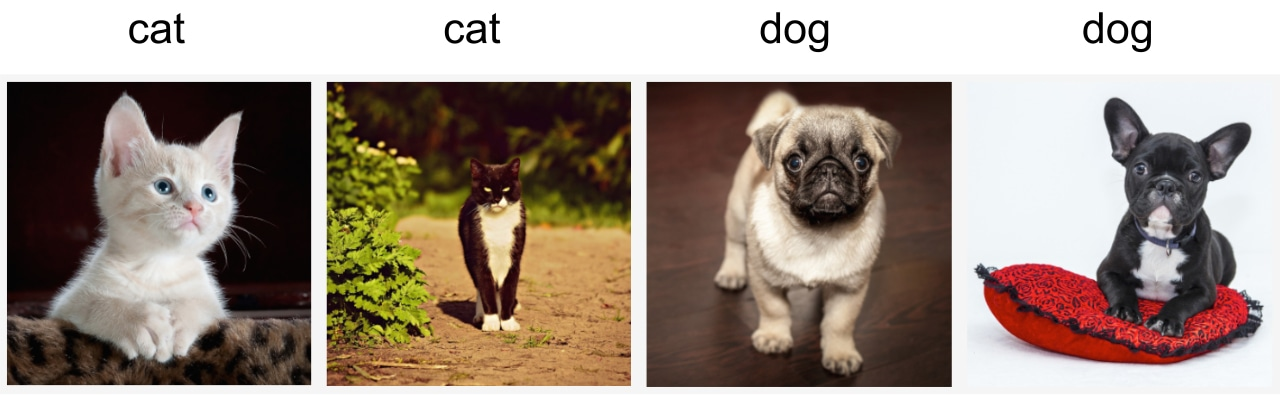
\includegraphics[scale=0.2]{../Images/cat-dog-train.jpg}
    \caption{Train Images}
    \label{fig:Train Images}
\end{figure}

\begin{figure}
    \centering
    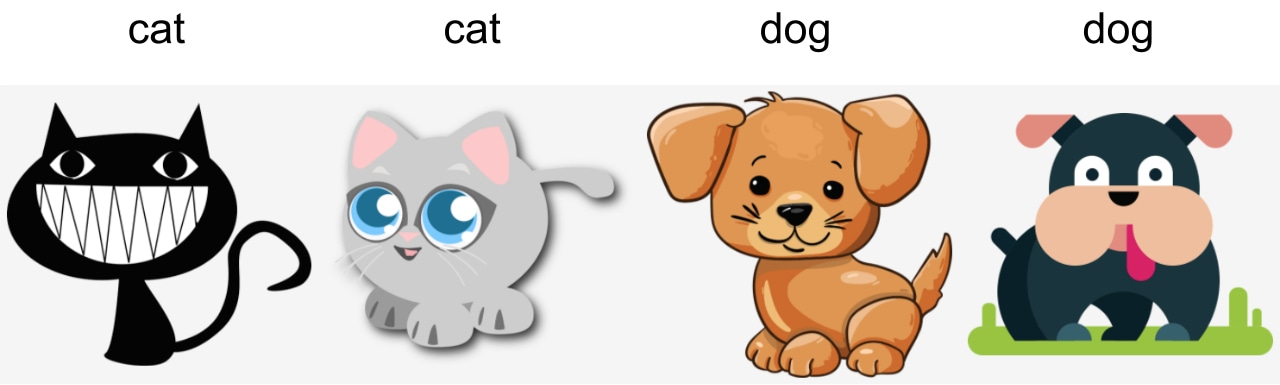
\includegraphics[scale=0.2]{../Images/cat-dog-test.jpg}
    \caption{Test Images}
    \label{fig:Test Images}
\end{figure}
\end{frame}

\section{Data Augmentation}
\begin{frame}{Data Augmentation}
\textbf{Data Augmentation:}\\
\qquad Data Augmentation is the process of increasing the amount and diversity of data. We do not collect new data, rather we transform the already present data. Data Augmentation is a natural and sometimes effective approach to learning robust models.\\ \qquad Examples of data augmentation include Adversarial Training, applying Image Transformations to the training data, such as flipping, cropping, adding Random Noise, and even stylized image transformation.
\end{frame}

\section{Gaussian Data Augmentation and Adversarial Training}
\begin{frame}[allowframebreaks]{Gaussian Data Augmentation and Adversarial Training}
\textbf{Gaussian Data Augmentation:}\\
\qquad Gaussian Data Augmentation[allowframebreaks] Technique integrates Signal-to-Noise Ratio (SNR) with an Additive White Gaussian Noise (AWGN) to generate derived data samples suited for multi-class classification in various Deep Neural Networks Models. 

\vspace{0.2in}

\textbf{Adversarial Training:}\\
\qquad The process of training the model on adversarially perturbed examples from the training set in the context of Regularization i.e inorder to reduce error on Test set. Adversarial training discourages this highly sensitive locally linear behavior by encouraging the network to be locally constant in the neighborhood of the training data. This can be seen as a way of explicitly introducing a local constancy prior into supervised neural nets.

\framebreak

\textbf{Examples of Adversarial Example Generation:}\\
\begin{figure}
    \centering
    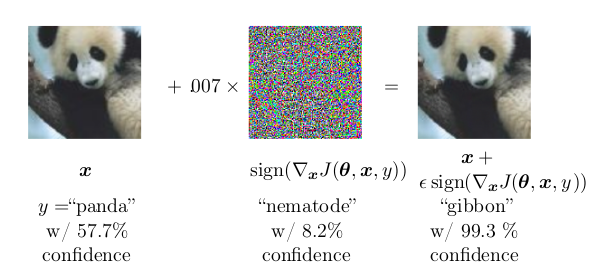
\includegraphics[scale=0.4]{../Images/Adversarial Training.png}
    \caption{A demonstration of adversarial example generation applied to GoogLeNet on ImageNet. By adding an imperceptibly small vector whose elements are equal to the sign of the elements of the gradient of the cost function with respect to the input, we can change GoogLeNet’s classification of the Image. (Source: \href{https://www.deeplearningbook.org/}{Deep Learning Book})}
    \label{fig:my_label}
\end{figure}
\end{frame}

\section{2D-Gaussian Distribution}
\begin{frame}[allowframebreaks]{2D-Gaussian Distribution}
\begin{figure}[ht]
    \begin{minipage}[b]{0.45\textwidth}
        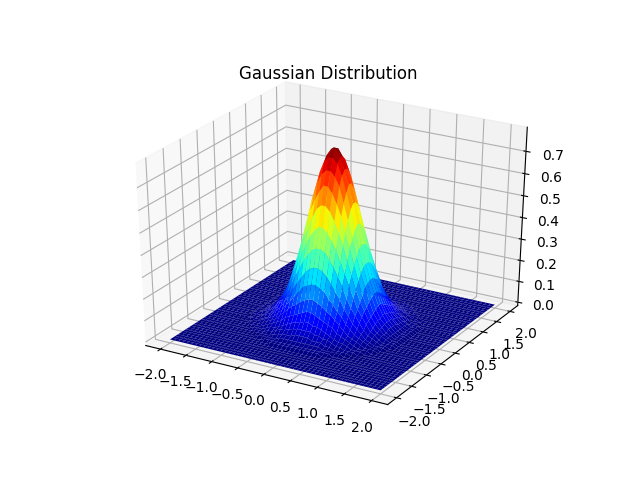
\includegraphics[scale=0.35]{../Images/Gaussian.png}
        \caption{2D-Gaussian Distribution}
        \label{fig:GD}
    \end{minipage}
    \begin{minipage}[b]{0.45\textwidth}
        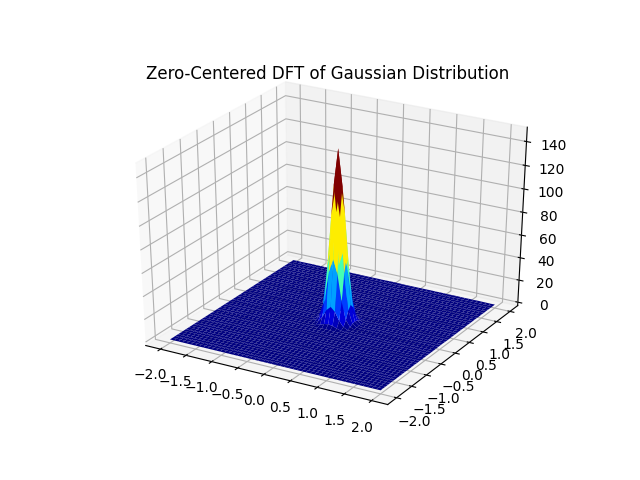
\includegraphics[scale=0.35]{../Images/ZeroCentered_Gaussian_DFT.png}
        \caption{DFT of 2D-Gaussian Distribution}
        \label{fig:DGD}
    \end{minipage}
\end{figure}
\framebreak
\begin{figure}[ht]
    \begin{minipage}[b]{0.45\textwidth}
        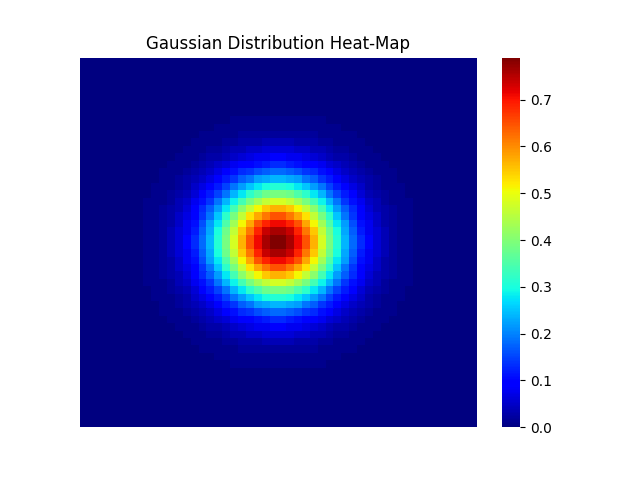
\includegraphics[scale=0.35]{../Images/Gaussian_HeatMap.png}
        \caption{Heat-Map of 2D-Gaussian}
        \label{fig:GDH}
    \end{minipage}
    \begin{minipage}[b]{0.45\textwidth}
        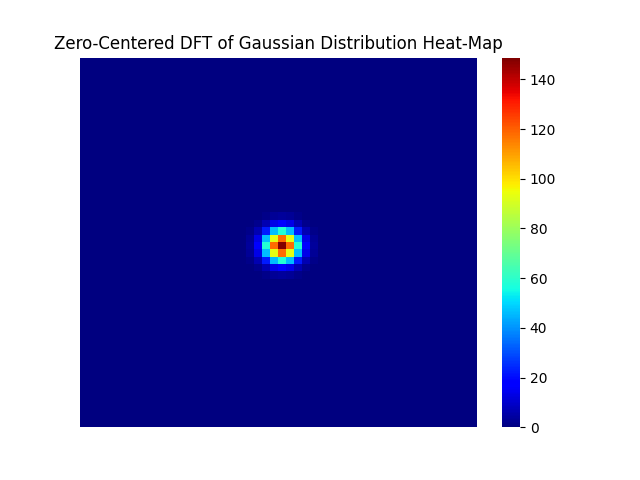
\includegraphics[scale=0.35]{../Images/ZeroCentered_Gaussian_DFT_HeatMap.png}
        \caption{Heat-Map of DFT of 2D-Gaussian}
        \label{fig:DGDH}
    \end{minipage}
\end{figure}
\end{frame}

\section{Hypothesis and Solution}
\begin{frame}{Hypothesis and Solution}
\textbf{Hypothesis:}\\
\qquad Operating Hypothesis of the paper is that the frequency information of these different corruptions offers an explanation of many of these observed trade-offs. Through extensive experiments involving perturbations in the Fourier domain, it is demonstrated that Augmentation Procedures like Gaussian Data Augmentation and Adversarial Training bias the model towards utilizing \textbf{Low Frequency Information} in the Input i.e if Input has low frequency content, corruptions with high frequencies increase the Robustness of Model while low frequency corruptions degrade the performance of model.\\
\vspace{0.2in}
\textbf{Solution:}\\
\qquad More diverse Data Augmentation Procedures could be leveraged to mitigate the trade-offs called \textbf{AutoAugment}. \textbf{AutoAugment} Data Augmentation achieves state-of-the art results on the CIFAR-10-C benchmark and ImageNet-C
\end{frame}

\section{Investigation}
\begin{frame}{Investigation}
\textbf{Gaussian Data Augmentation:}\\
\qquad A parameter $\sigma$ for the following operation: In each iteration, we add i.i.d. Gaussian Noise $\mathcal{N}(0,\tilde{\sigma}^2)$ to every pixel in all the images in the training batch, where $\tilde{\sigma}$ is chosen uniformly at random from $[0, \sigma]$.  When Gaussian Data Augmentation is used, $\sigma = 0.1$ for CIFAR-10 and $\sigma = 0.4$ for ImageNet.
\vspace{0.1in}
\textbf{Sensitivity of Models:}\\
In-order to investigate sensitivity of models towards corruptions, we define a $U_{i,j} \in R^{d_1 \times d_2}$ called 2D-Fourier Basis Matrices which have the following properties:\\
\begin{enumerate}
    \item $||U_{i,j}|| = 1$
    \item $\mathcal{F}(U_{i,j})$ only has up to two non-zero elements located at (i, j) and the its symmetric coordinate with respect to the image center.
\end{enumerate}
\end{frame}

\end{document}
